\documentclass[%
%%% PARA ESCOLHER O ESTILO TIRE O SIMBOLO %(COMENTÁRIO)
%SemVinculoColorido,
%SemFormatacaoCapitulo,
%SemFolhaAprovacao,
%SemImagens,
%CitacaoNumerica, %% o padrão é citação tipo autor-data
%PublicacaoDissOuTese, %% (é também o "default") com ficha catal. e folha de aprovação em branco. Caso tenha lista de símbolos e lista de siglas e abreviaturas retirar os comentários dos arquivos siglas.tex e abreviaturasesiglas.tex. Retirar também os comentários indicados nesse arquivo, nos includes
PublicacaoArtigoOuRelatorio, %% texto sequencial, sem quebra de páginas nem folhas em branco
%PublicacaoProposta, %% igual tese/dissertação, mas sem ficha catal. e fol. de aprov.
%PublicacaoLivro, %% com capítulos
%PublicacaoLivro,SemFormatacaoCapitulo, %% sem capítulos
english,portuguese %% para os documentos em Português com abstract.tex em Inglês
%portuguese,english %% para os documentos em Inglês com abstract.tex em Português
,LogoINPE% comentar essa linha para fazer aparecer o logo do Governo
%,CCBYNC	% as opções de licença são: CCBY, CCBYSA, CCBYND, CCBYNC, CCBYNCSA, CCBYNCND, GPLv3 e INPECopyright
]{tdiinpe}
%]{../../../../../iconet.com.br/banon/2008/03.25.01.19/doc/tdiinpe}

% PARA EXIBIR EM ARIAL TIRAR O COMENTÁRIO DAS DUAS LINHAS SEGUINTES
%\renewcommand{\rmdefault}{phv} % Arial
%\renewcommand{\sfdefault}{phv} % Arial

% PARA PUBLICAÇÕES EM INGLÊS:
% renomear o arquivo: abnt-alf.bst para abnt-alfportuguese.bst
% renomear o arquivo: abnt-alfenglish.bst para abnt-alf.bst


%%%%%%%%%%%%%%%%%%%%%%%%%%%%%%%%%%%%%%%%%%%%%
%%% Pacotes já previamente carregados:      %
%%%%%%%%%%%%%%%%%%%%%%%%%%%%%%%%%%%%%%%%%%%%%%%%%%%%%%%%%%%%%%%%%%%%%%%%
%%% ifthen,calc,graphicx,color,inputenc,babel,hyphenat,array,setspace, %
%%% bigdelim,multirow,supertabular,tabularx,longtable,lastpage,lscape, %
%%% rotate,caption2,amsmath,amssymb,amsthm,subfigure,tocloft,makeidx,  %
%%% eso-pic,calligra,hyperref,ae,fontenc                               %
%%%%%%%%%%%%%%%%%%%%%%%%%%%%%%%%%%%%%%%%%%%%%%%%%%%%%%%%%%%%%%%%%%%%%%%%
%%% insira neste campo, comandos de LaTeX %%%
%%% \usepackage{_exemplo_}
% etc.
%%%%%%%%%%%%%%%%%%%%%%%%%%%%%%%%%%%%%%%%%%%%%

%\watermark{Revisão No. ##} %% use o comando \watermark para identificar a versão de seu documento
%% comente este comando quando for gerar a versão final
% Alterando Numeracao dos Capitulos (numero romano) e Secoes (alfabeto)
\renewcommand{\thechapter}{\Roman{chapter}}
\renewcommand{\thesection}{\alph{section})}
\usepackage{rotating}
\usepackage{dsfont}
\usepackage{comment}

\usepackage{tikz}
\usetikzlibrary{shapes,backgrounds}
\def\firstcircle{(90:1.cm) circle (2.cm)}
\def\secondcircle{(210:1.75cm) circle (2.5cm)}
\def\thirdcircle{(330:1.cm) circle (2.25cm)}

\newcommand{\latex}{\LaTeX\xspace}

%\usepackage{float}
%\usepackage{scrextend}
%\graphicspath{ {.} }
%\pagenumbering{gobble}
\usepackage{listings}
\usepackage{booktabs}
\lstset{language=c} 
\lstset{language=C, literate={-}{-}1}

\usepackage{xcolor}

\definecolor{codegreen}{rgb}{0,0.6,0}
\definecolor{codegray}{rgb}{0.3,0.3,0.3}
\definecolor{codepurple}{rgb}{0.58,0,0.82}
\definecolor{backcolour}{rgb}{0.95,0.95,0.92}

\lstdefinestyle{mystyle}{
    backgroundcolor=\color{backcolour},   
    commentstyle=\color{codegreen},
    keywordstyle=\color{magenta},
    numberstyle=\tiny\color{codegray},
    stringstyle=\color{codepurple},
    basicstyle=\ttfamily\footnotesize,
    breakatwhitespace=false,         
    breaklines=true,                 
    captionpos=b,                    
    keepspaces=true,                 
    numbers=left,                    
    numbersep=5pt,                  
    showspaces=false,                
    showstringspaces=false,
    showtabs=false,                  
    tabsize=2
}

\lstdefinestyle{mystyle2}{
    backgroundcolor=\color{backcolour},   
    commentstyle=\color{codegreen},
    keywordstyle=\color{magenta},
    stringstyle=\color{codepurple},
    basicstyle=\ttfamily\footnotesize,
    breakatwhitespace=false,         
    breaklines=true,                 
    captionpos=b,                    
    keepspaces=true,                                             
    showspaces=false,                
    showstringspaces=false,
    showtabs=false,                  
    tabsize=2
}

\DeclareMathOperator*{\di}{\mathrm{d}\!}
\def\at{
  \left.
  \vphantom{\int}
  \right|
}

\renewcommand{\arraystretch}{1.2}
%\lstset{style=mystyle}
%\lstset{inputencoding=utf8/latin1}

%%%%%%%%%%%%%%%%%%%CAPA%%%%%%%%%%%%%%%%%%%%%%%%%%%%%%%%
%\serieinpe{INPE-NNNNN-TDI/NNNN} %% não mais usado

\titulo{Avaliação da Capacidade de Vetorização de Três Compiladores C Disponíveis no Supercomputador Santos Dumont}
\title{Avaliação da Capacidade de Vetorização de Três Compiladores C Disponíveis no Supercomputador Santos Dumont} %% 
\author{Leonardo Sattler Cassará} %% coloque o nome do(s) autor(es)
\descriccao{Projeto Final apresentado aos Professores Celso L. Mendes e Stephan Stephany como parte da avaliação do curso CAP-399.}
\repositorio{} %% repositório onde está depositado este documento - na omissão, será preenchido pelo SID
\tipoDaPublicacao{}	%% tipo da publicação (NTC, RPQ, PRP, MAN, PUD, TDI, TAE e PRE) na ausência do número de série INPE, caso contrário deixar vazio
\IBI{} %% IBI (exemplo: J8LNKAN8PW/36CT2G2) quando existir, caso contrário o nome do repositório onde está depositado o documento

\date{18 de dezembro de 2020}%ano da publicação

%%%%%%%%%%%%%%%%%%%%%%%%%%VERSO DA CAPA%%%%%%%%%%%%%%%%%%%%%%%%%%%%%%%%%%%%%%%%%%%%%%%
\tituloverso{}
\descriccaoverso{}

\descriccaoversoA{}

%%%%%%%%%%%%%%%%%%%FOLHA DE ROSTO

%%%%%%%%%%%%%%%FICHA CATALOGRÁFICA
%% NÃO PREENCHER - SERÁ PREENCHIDO PELO SID

\cutterFICHAC{Cutter}
\autorUltimoNomeFICHAC{Sobrenome, Nomes} %% exemplo: Fuckner, Marcus André
\autorFICHAC {Nome Completo do Autor1; Nome Completo do Autor2} %% Campo opcional (se não usado prevalece \author)
\tituloFICHAC{Titulo da publicação}
\instituicaosigla{INPE}
\instituicaocidade{São José dos Campos}
\paginasFICHAC{\pageref{numeroDePáginasDoPretexto} + \pageref{LastPage}} %% número total de páginas
%\serieinpe{INPE-00000-TDI/0000} %% não mais usado
\palavraschaveFICHAC{1.~Palavra chave. 2.~Palavra chave 3.~Palavra chave. 4.~Palavra chave. 5.~Palavra chave  I.~\mbox{Título}.} %% recomenda-se pelo menos 5 palavras-chaves - \mbox{} é para evitar hifenização 
\numeroCDUFICHAC{000.000} %% número do CDU 

% Nota da ficha (para TD)
\tipoTD{Dissertação ou Tese} % Dissertação ou Tese
\cursoFA{Mestrado ou Doutorado em Nome do Curso}
\instituicaoDefesa{Instituto Nacional de Pesquisas Espaciais}
\anoDefesa{AAAA} % ano de defesa 
\nomeAtributoOrientadorFICHAC{Orientador}	% pode ser: Orientador, Orientadora ou Orientadores
\valorAtributoOrientadorFICHAC{José da Silva} % nome(s) completo(s)

%%%%%%%%%%%%%%%FOLHA DE APROVAÇAO PELA BANCA EXAMINADORA
\tituloFA{\textbf{ATENÇÃO! A FOLHA DE APROVAÇÃO SERÁ INCLUIDA POSTERIORMENTE.}}
%\cursoFA{\textbf{}}
\candidatoOUcandidataFA{}
\dataAprovacaoFA{}
\membroA{}{}{}
\membroB{}{}{}
\membroC{}{}{}
\membroD{}{}{}
\membroE{}{}{}
\membroF{}{}{}
\membroG{}{}{}
\ifpdf

%%%%%%%%%%%%%%NÍVEL DE COMPRESSÃO {0 -- 9}
\pdfcompresslevel 9
\fi
%%% define em 80% a largura das figuras %%%
\newlength{\mylenfig} 
\setlength{\mylenfig}{0.8\textwidth}
%%%%%%%%%%%%%%%%%%%%%%%%%%%%%%%%%%%%%%%%%%%

%%%%%%%%%%%%%%COMANDOS PESSOAIS
\newcommand{\vetor}[1]{\mathit{\mathbf{#1}}} %% faça as modificações pertinentes no arquivo configuracao.tex

\makeindex  %% não alterar, gera INDEX, caso haja algum termo indexado no texto

\begin{document} %% início do documento %% não mexer

%\marcaRegistrada{}	% comando opcional usado para informar abaixo da ficha catalográfica sobre marca registrada
%\marcaRegistrada{Informar aqui sobre marca registrada (a modificação desta linha deve ser feita no arquivo publicacao.tex).}

\maketitle  %% não alterar, gera páginas obrigatórias (folha de rosto, ficha catalográfica e folha de aprovação), automaticamente
\pagenumbering{roman}
%%% Comente as linhas opcionais abaixo caso não as deseje
%\include{./docs/epigrafe} %% Opcional
%\include{./docs/dedicatoria} %% Opcional
%\include{./docs/agradecimentos} %% Opcional
%\include{./docs/resumo} %% obrigatório
%%%%%%%%%%%%%%%%%%%%%%%%%%%%%%%%%%%%%%%%%%%%%%%%%%%%%%%%%%%%%%%%%%%%%%%%%%%%%%%%
% RESUMO %% obrigatório

\begin{resumo}

No presente trabalho, os compiladores \texttt{Intel v.19.1}, \texttt{PGI v.19.4} e \texttt{GNU v.8.3} são avaliados quanto à capacidade de vetorização. Foi utilizada uma versão ligeiramente modificada da coleção de testes TSVC (Test Suite for Vectorizing Compilers) descrita em \citeonline{maleki2011evaluation}. Este manuscrito está dividido em três seções: na Seção I, os resultados da bateria de testes são apresentados, caracterizando os ganhos e desempenhos obtidos pela vetorização de cada compilador; na Seção II, as flags de compilação são alteradas de modo a buscar \textit{Speedups} superiores aos obtido durante os testes da primeira seção; as conclusões são apresentadas na Seção III.

%% neste arquivo resumo.tex
%% o texto do resumo e as palavras-chave têm que ser em Português para os documentos escritos em Português
%% o texto do resumo e as palavras-chave têm que ser em Inglês para os documentos escritos em Inglês
%% os nomes dos comandos \begin{resumo}, \end{resumo}, \palavraschave e \palavrachave não devem ser alterados

\hypertarget{estilo:resumo}{} %% uso para este Guia

%\palavraschave{%
%	\palavrachave{Wavelet analysis}%
%	\palavrachave{Gapped data}%
%	\palavrachave{Numerical methods}%
%	\palavrachave{Lomb-Scargle periodogram}%
%	\palavrachave{Spectral analysis}%
%}
 
\end{resumo} %% obrigatório

\includeListaTabelas %% obrigatório caso haja mais de 3 tabelas, gerado automaticamente
\includeListaFiguras %% obrigatório caso haja mais de 3 figuras, gerado automaticamente

%%%%%%%%%%%%%%%%%%%%%%%%%%%%%%%%%%%%%%%%%%%%%%%%%%%%%%%%%%%%%%%%%%%%%%%%%%%%%%%%%
%abreviaturas e siglas  %% opcional, mas recomendado

\begin{abreviaturasesiglas}  %% insira abaixo suas abreviaturas conforme o modelo.
\end{abreviaturasesiglas}
 %% opcional %% altere o arquivo siglaseabreviaturas.tex

%\include{./docs/simbolos} %% opcional %% altere o arquivo simbolos.tex

\includeSumario  %% obrigatório, gerado automaticamente

\newpage
%%%%%%%%%%%%%%%%%%%%%%%%%%%%%%%%%%%%%%%%%%%%%%%%%%%%%%%%%%%%%%%%%%%%%%%%%%%%%%%

\chapter*{PREFÁCIO}
\addcontentsline{toc}{chapter}{PREFÁCIO}% \protect\numberline{}

Os resultados deste trabalho foram gerados no supercomputador Santos Dumont sob usuário \textit{leonardo.cassara}. Todos os arquivos referentes à geração dos resultados se encontram divididos em seis diretórios: três referentes à Seção \ref{chp:1} deste projeto, \texttt{GCC\_1}, \texttt{ICC\_1}, \texttt{PGI\_1} (e referentes aos compiladores \texttt{GNU v.8.3}, \texttt{Intel v.19.1} e \texttt{PGI v.19.4}, respectivamente), e três que dizem respeito à Seção \ref{chp:2} deste projeto, \texttt{GCC\_2}, \texttt{ICC\_2}, \texttt{PGI\_2} (e referentes aos mesmos compiladores). Cada diretório contém seus respectivos scripts de submissão, outputs, makefiles, os programas de teste e outros arquivos necessários para a geração dos resultados. Tais diretórios se encontram no seguinte local do Santos Dumont:
\begin{lstlisting}[language=bash,style=mystyle2]
/scratch/padinpe/leonardo.cassara/PSMP_scratch/Projeto/
\end{lstlisting}
%\vspace{-3mm}

A análise dos resultados foi realizada localmente (em um computador pessoal) através da linguagem \texttt{Python}, com uso das bibliotecas \texttt{numpy} e \texttt{pandas} para geração das tabelas e \texttt{matplotlib} para criação das figuras. Todos os arquivos referentes à análise dos resultados estão no repositório deste projeto. O conteúdo do repositório é descrito abaixo:

\begin{itemize}
\item pasta \textbf{sdumont}: cópia dos seis diretórios presentes no Santos Dumont, disponibilizando os resultados para o público sem acesso ao supercomputador.

\item pasta \textbf{Relatorio}: contém os arquivos \LaTeX  \hspace{0.09mm} utilizados para a geração deste manuscrito.

\item \textit{data\_handler.py}: script de análise dos resultados, que gera as tabelas e as figuras presentes neste manuscrito, bem como uma planilha com os resultados.

\item \textit{data\_comp.py}: script para comparação dos resultados, que gera tabelas com a alteração relativa entre as quantidades contrastadas.

\item \textit{stats\_tools.py}: script para cálculo das estatística dos resultados, utilizado pelos scripts \textit{data\_handler.py} e \textit{data\_comp.py}.

\item \textit{results1.xlsx}: planilha contendo os resultados apresentados nas Tabelas \ref{tab:a} e \ref{tab:b} deste manuscrito.

\item \textit{results2.xlsx}: planilha contendo os resultados da Seção \ref{chp:2}.
\end{itemize} 
\clearpage
\inicioIntroducao %% não altere este comando

\newpage
%%%%%%%%%%%%%%%%%%%%%%%%%%%%%%%%%%%%%%%%%%%%%%%%%%%%%%%%%%%%%%%%%%%%%%%%%%%%%%%

\chapter{APRESENTAÇÃO DOS RESULTADOS}
\label{chp:1}

A bateria de testes realizada neste projeto consistiu de seis execuções: duas para cada um dos três compiladores, sendo a primeira com e a segunda sem vetorização ativada durante a compilação (ver Tabela \ref{tab:2_flags} para detalhes das flags de compilação utilizadas em cada caso). Os resultados obtidos na bateria de testes são apresentados a seguir para os três compiladores testados: \texttt{ICC} (versão 19.1), \texttt{PGI} (versão 19.1) e \texttt{GCC} (versão 8.3).

\section{Tempos de cada execução}

A Tabela \ref{tab:a} exibe os tempos obtidos em dez dos 151 loops de teste (cinco primeiros e cinco últimos) durante as seis execuções da bateria de testes.

\begin{table}[H]
\center
\caption{Tempos de execução em segundos obtidos em dez dos 151 loops da bateria de testes.} 
\begin{tabular}{@{}l l l l l l l l l l@{}}
\toprule
% & & \multicolumn{3}{@{}c@{}}{Exercício 1 -- \texttt{prog.c}} & & \multicolumn{3}{@{}c@{}}{Exercício 2 -- \texttt{prog2.c}}\\
%\cmidrule{3-5} \cmidrule{7-9}
 & & \multicolumn{8}{@{}c@{}}{Tempos de execução [s]} \\
 \cmidrule{3-10}
 & & \multicolumn{2}{@{}c@{}}{\texttt{ICC}} & & \multicolumn{2}{@{}c@{}}{\texttt{PGI}} & &  \multicolumn{2}{@{}c@{}}{\texttt{GCC}} \\
\cmidrule{3-4} \cmidrule{6-7} \cmidrule{9-10}
Loop & & Não-vet. & Vet.  & &  Não-vet. & Vet.  & &  Não-vet. & Vet. \\
\midrule
S000  & &    0.414  &   0.169  & &    0.360 &    0.338   & &   0.540 &    0.170 \\
S111  & &   0.274   &  0.269   & &   0.269  &   0.290    & &  0.286  &   0.252 \\
S1111 & &   0.566   &  0.371   & &   0.581  &   0.580    & &  0.680  &   0.339 \\
S112  & &   0.628   &  0.631   & &   0.295  &   0.334    & &  0.811  &   0.436 \\
S1112 & &   0.616   &  0.243   & &   0.232  &   0.267    & &   0.808 &    0.329 \\
\multicolumn{1}{c}{\vdots} & & \multicolumn{1}{c}{\vdots}  & \multicolumn{1}{c}{\vdots}   & & \multicolumn{1}{c}{\vdots} & \multicolumn{1}{c}{\vdots}     & & \multicolumn{1}{c}{\vdots} & \multicolumn{1}{c}{\vdots} \\
vpvpv  & &  1.150  &  0.627   & &   0.664  &  0.628   & &  1.257   &  0.684 \\
vtvtv  & &  1.156  &  0.630   & & 0.673   &  0.630    & &  1.268   &  0.685 \\
vsumr  & &  2.005  &  0.418   & &  4.006  &   0.502   & &   4.009  &   4.007 \\
vdotr  & &  2.055  &  0.904   & &  4.013  &   0.890   & &   4.013  &   4.010 \\
vbor   & &  0.133  &  0.089   & &  0.358  &   0.045   & &   0.358  &   0.090 \\
\bottomrule
\end{tabular}
\label{tab:a}
\end{table}

A Figura \ref{fig:a} exibe os histogramas dos tempos de execução obtidos com os três compiladores testados, para compilações sem vetorização (barras de cor laranja) e com vetorização (barras de cor azul). Os histogramas também apresentam as estatísticas de cada caso.

\begin{figure}[ht!]
	\vspace{0mm}	% acrescentar o espaçamento vertical apropriado entre o título e a borda superior da figura
	\begin{center}
		\resizebox{\textwidth}{!}{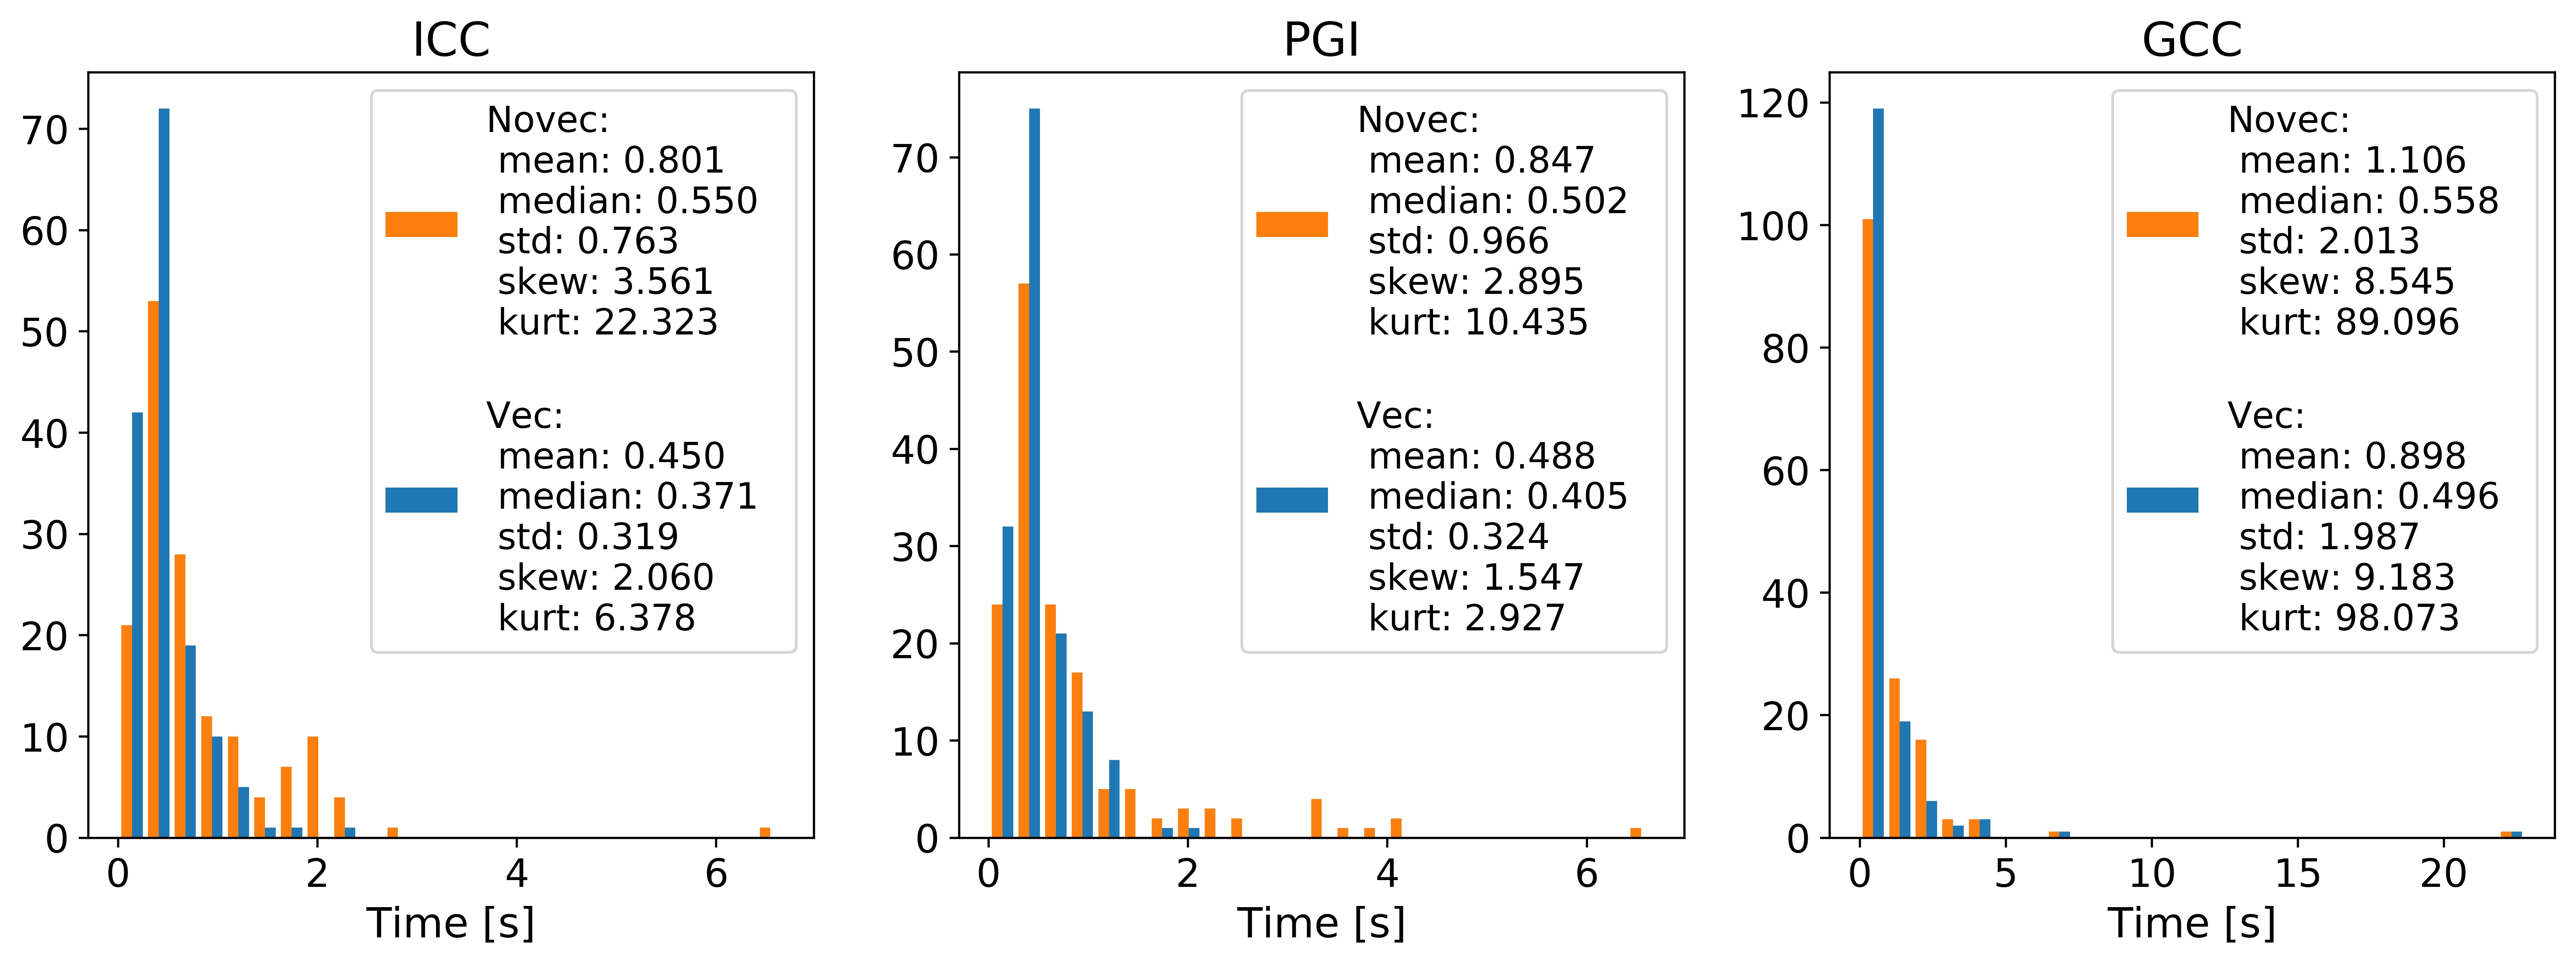
\includegraphics{Figuras/stats.jpg}}		
	\end{center}
	\vspace{2mm}	% acrescentar o espaçamento vertical apropriado entre a borda inferior da figura e a legenda ou a fonte quando não há legenda (o valor pode ser negativo para subir)
	\caption{Histogramas dos resultados obtidos nas execuções sem vetorização (barras de cor laranja) e com vetorização (barras de cor azul) dos três compiladores testados. O número de bins é igual a 25. As estatísticas de cada distribuição estão indicadas, incluindo a média (\textsf{mean}), mediana (\textsf{median}), o desvio padrão (\textsf{std}), o coeficiente de assimetria (\textsf{skew}) e o coeficiente de curtose (\textsf{kurt}).}
	\legenda{}	% legenda - para deixar sem legenda usar comando \legenda{} (nunca deve-se comentar o comando \legenda)
	\label{fig:a}
%	\FONTE{FOnte da imagem (se necessário).}	% fonte consultada (elemento obrigatório, mesmo que seja produção do próprio autor)
\end{figure}


\section{\textit{Speedups} de cada execução}

A Tabela \ref{tab:b} apresenta os \textit{Speedups} de dez dos 151 loops para os três compiladores testados, obtidos através da Tabela \ref{tab:a}.

\begin{table}[H]
\center
\caption{\textit{Speedups} de dez dos 151 loops da bateria de testes.} 
\begin{tabular}{@{}l l l l l@{}}
\toprule
 & & \multicolumn{3}{@{}c@{}}{\textit{Speedups}}\\
 \cmidrule{3-5} 
Loop & & \texttt{ICC} & \texttt{PGI} &  \texttt{GCC} \\
\midrule
S000    & &   2.45    &   1.07   &   3.18 \\
S111    & &   1.02    &   0.93   &   1.13 \\
S1111   & &   1.53    &   1.00   &   2.01 \\
S112    & &   1.00    &   0.88   &   1.86 \\
S1112   & &   2.53    &   0.87   &   2.46 \\
\multicolumn{1}{c}{\vdots} & & \multicolumn{1}{c}{\vdots} & \multicolumn{1}{c}{\vdots} & \multicolumn{1}{c}{\vdots} \\
vpvpv    & &   1.83   &   1.06     &   1.84 \\
vtvtv    & &   1.83   &   1.07     &   1.85 \\
vsumr    & &   4.80   &   7.98     &   1.00 \\
vdotr    & &   2.27   &   4.51     &   1.00 \\
vbor     & &   1.49   &   7.96     &   3.98 \\
\bottomrule
\end{tabular}
\label{tab:b}
\end{table}


\section{\textit{Speedups} médios}

A partir da Tabela \ref{tab:b}, foi calculado o \textit{Speedup} médio de cada compilador:

\begin{table}[H]
\center
\caption{Médias dos 151 \textit{Speedups} resultantes dos testes dos três compiladores.} 
\begin{tabular}{@{}l l l l@{}}
\toprule
& \texttt{ICC} & \texttt{PGI} &  \texttt{GCC} \\
\midrule
\textit{Speedup} médio & 1.79 & 1.96 & 1.41 \\ 
\bottomrule
\end{tabular}
\label{tab:c}
\vspace{-3mm}
\end{table}

\section{Tempos totais}

A partir da Tabela \ref{tab:a}, foi calculado o tempo total de cada execução da bateria de testes:


\begin{table}[H]
\center
\caption{Somas dos tempos obtidos nos 151 loops das seis execuções.} 
\begin{tabular}{@{}l l l l l l l l l@{}}
\toprule
& \multicolumn{2}{@{}c@{}}{\texttt{ICC}} & & \multicolumn{2}{@{}c@{}}{\texttt{PGI}} & &  \multicolumn{2}{@{}c@{}}{\texttt{GCC}} \\
\cmidrule{2-3} \cmidrule{5-6} \cmidrule{8-9}
& Não-vet. & Vet.  & &  Não-vet. & Vet.  & &  Não-vet. & Vet. \\
\midrule
Tempo total [s] & 120.891 &  67.916 & & 127.894  &  73.688  & &  166.968  &  135.628 \\
\bottomrule
\end{tabular}
\label{tab:d}
\vspace{-3mm}
\end{table}

Com os valores da Tabela \ref{tab:d}, os \textit{Speedups} dos compiladores \texttt{ICC}, \texttt{PGI} e \texttt{GCC} são, respectivamente, 1.78, 1.74 e 1.23 (comparar com os valores da Tabela \ref{tab:c}).

\section{Número de loops vetorizados e não-vetorizados}

Através da Tabela \ref{tab:b}, e utilizando o limiar de 1.5 adotado em \citeonline{maleki2011evaluation}, foi obtido o número de loops vetorizados e não-vetorizados pelos três compiladores testados:


\begin{table}[H]
\center
\caption{Número de loops vetorizados e não-vetorizados (dentre os 151 loops de teste) por cada compilador.} 
\begin{tabular}{@{}l l l l l l l l@{}}
\toprule
\multicolumn{2}{@{}c@{}}{\texttt{ICC}} & & \multicolumn{2}{@{}c@{}}{\texttt{PGI}} & &  \multicolumn{2}{@{}c@{}}{\texttt{GCC}} \\
\cmidrule{1-2} \cmidrule{4-5} \cmidrule{7-8}
Não-vet. & Vet.  & &  Não-vet. & Vet.  & &  Não-vet. & Vet. \\
\midrule
57    &    94     &&     101     &    50     &&     108   & 43 \\
\bottomrule
\end{tabular}
\label{tab:e}
\end{table}


\section{Loops não-vetorizados}

Considerando o mesmo limiar de 1.5, foi determinado o número de loops não-vetorizados por nenhum dos três compiladores testados. Ao todo, 45 loops nunca foram vetorizados durante a bateria de testes. Tais loops são mostrados a seguir:

\begin{table}[H]
\center
\caption{Nomes dos loops que não foram vetorizados por nenhum compilador. O total é igual a 45.} 
\begin{tabular}{@{}l l l l l l l l l@{}}
\toprule
S111 & S1113 & S114 & S1115 & S118 & S123 & S126 & S141 & S161 \\
S162 & S171 & S172 & S232 & S1232 & S252 & S255 & S256 & S257 \\
S258 & S277 & S281 & S293 & S2101 & S2111 & S31111 & S3110 & S3112 \\
S321 & S322 & S323 & S332 & S341 & S342 & S343 & S353 & S481 \\
S482 & S491 & S4112 & S4113 & S4114 & S4115 & S4116 & vag & vas \\
\bottomrule
\end{tabular}
\label{tab:f}
\end{table}

A Figura \ref{fig:f} resume a distribuição de loops vetorizados e não-vetorizados pelos três compiladores ao longo dos testes.


\begin{figure}[ht!]
	\vspace{0mm}	% acrescentar o espaçamento vertical apropriado entre o título e a borda superior da figura
	\begin{center}
\begin{tikzpicture}

\draw \firstcircle (90:3.5) node[text=black] {GCC};

\draw   (90:2.1) node[text=black] {4};

\draw   (0:0) node[text=black] {10};

\draw   (145:1.7) node[text=black] {25};

\draw   (40:1.7) node[text=black] {4};

\draw \secondcircle (210:4.5) node [text=black,below left] {ICC};

\draw   (210:3) node[text=black] {27};

\draw   (270:1.8) node[text=black] {32};

\draw \thirdcircle (330:3.5) node [text=black,below right] {PGI};

\draw   (330:2.5) node[text=black] {4};

%\draw (-6.5,3.5) circle (1) node [text=black] {45};

\draw (-5.6,-4) rectangle (4.2,4.5);% node [text=black,above left] {Vetorizados};

\draw (-4,2.8) circle (1);% node [text=black,above left] {Não-vetorizados};

\draw (-3.9,4.1) node[text=black] {Não-vetorizados};

%\draw (-4.7,2.6) rectangle (-2.2,3.9) node [text=black,above left] {Não-vetorizados};

\draw (-4,2.8) node[text=black] {45};

\end{tikzpicture}	
	\end{center}
	\vspace{2mm}	% acrescentar o espaçamento vertical apropriado entre a borda inferior da figura e a legenda ou a fonte quando não há legenda (o valor pode ser negativo para subir)
	\caption{Diagrama de Venn do número de loops vetorizados e não-vetorizados pelos compiladores \texttt{ICC}, \texttt{PGI} e \texttt{GCC} ao longo dos testes realizados.}
	\legenda{}	% legenda - para deixar sem legenda usar comando \legenda{} (nunca deve-se comentar o comando \legenda)
	\label{fig:f}
%	\FONTE{FOnte da imagem (se necessário).}	% fonte consultada (elemento obrigatório, mesmo que seja produção do próprio autor)
\end{figure}



%Citação dentro de parênteses: \cite{press1989fast} % com parenteses

%Citação fora de parênteses (na linha): \citeonline{frick1998wavelet} % sem parenteses



%\include{./docs/methods} 
\newpage
%%%%%%%%%%%%%%%%%%%%%%%%%%%%%%%%%%%%%%%%%%%%%%%%%%%%%%%%%%%%%%%%%%%%%%%%%%%%%%%

\chapter{BUSCANDO MAIORES \textit{SPEEDUPS}}
\label{chp:2}

A Tabela \ref{tab:2_flags} detalha as flags de compilação utilizadas para gerar os resultados das Seções \ref{chp:1} e \ref{chp:2}. A Figura \ref{fig:2_hist} ilustra os resultados das execuções com as novas flags. Os novos \textit{Speedups} médios calculados estão na Tabela \ref{tab:2_spedups}; os novos tempos totais estão na Tabela \ref{tab:2_tempos}; a Tabela \ref{tab:2_nloops} indica o número de loops vetorizados e não-vetorizados por cada compilador, com a informação de quantos loops a mais ou a menos foram vetorizados. Nas Tabelas \ref{tab:2_spedups} e \ref{tab:2_tempos} está indicada a alteração relativa $\delta$ das quantidades apresentadas com relação aos resultados da Seção \ref{chp:1}, definida por:

\begin{equation}
\delta = \frac{x_{II}-x_{I}}{x_{I}}, 
\end{equation}

sendo $x_{I}$ e $x_{II}$ os valores das quantidades pertinentes às Seções \ref{chp:1} e \ref{chp:2}, respectivamente. Ou seja, os valores de $x_{I}$ são adotados como referência para quantificar a performance das novas otimizações. 

\renewcommand{\arraystretch}{1.3}
\begin{table}[H]
\center
\caption{Flags de compilação utlizadas nas Seções \ref{chp:1} e \ref{chp:2}.} 
\begin{tabular}{@{}l | l c | c@{}}
\toprule
\multicolumn{2}{@{}l@{}}{ } & \multicolumn{2}{@{}c@{}}{Flags}\\
\cmidrule{2-4}
% -------------------------------
\multicolumn{2}{@{}l@{}}{\texttt{ICC}} &  Seção I & Seção II  \\
\hline  
Otimização base & & \multicolumn{2}{@{}c@{}}{\small \texttt{-std=c99 -O3}} \\
\hline
Vetorização & & \small (ativada via \texttt{-O3} da otim. base) & \small \texttt{-xSSE4.2} \\
\hline
Sem vetorização & & \multicolumn{2}{@{}c@{}}{\small \texttt{-no-vec}} \\
\hline
Relatório de vet. & & \multicolumn{2}{@{}c@{}}{\small \texttt{-qopt-report=2 -qopt-report-phase=vec}} \\
\midrule
% -------------------------------
\multicolumn{2}{@{}l@{}}{\texttt{PGI}} &  Seção I & Seção II  \\
\hline
Otimização base & & \small \texttt{-c99 -O3} & \small \texttt{-c99 -O3 -Mcache\_align} \\
\hline
Vetorização & & \small \texttt{-Mvect=sse} & \small \texttt{-Mvect=sse -Mvect=prefetch} \\
\hline
Sem vetorização & & \multicolumn{2}{@{}c@{}}{\small \texttt{-Mnovect}} \\
\hline
Relatório de vet. & & \multicolumn{2}{@{}c@{}}{\small \texttt{-Minfo}} \\
\midrule
% -------------------------------
\multicolumn{2}{@{}l@{}}{\texttt{GCC}} &  Seção I & Seção II  \\
\hline
Otimização base & & \small \texttt{-O3} & \small \texttt{-O3 -ffast-math} \\
\hline
Vetorização & & \multicolumn{2}{@{}c@{}}{\small \texttt{-ftree-vectorize}} \\
\hline
Sem vetorização & & \multicolumn{2}{@{}c@{}}{\small \texttt{-fno-tree-vectorize}} \\
\hline
Relatório de vet. & & \multicolumn{2}{@{}c@{}}{\small \texttt{-fdump-tree-vect-blocks=report.dump}} \\
\bottomrule
\end{tabular}
\label{tab:2_flags}
\end{table}


\begin{figure}[ht!]
	\vspace{0mm}	% acrescentar o espaçamento vertical apropriado entre o título e a borda superior da figura
	\begin{center}
		\resizebox{\textwidth}{!}{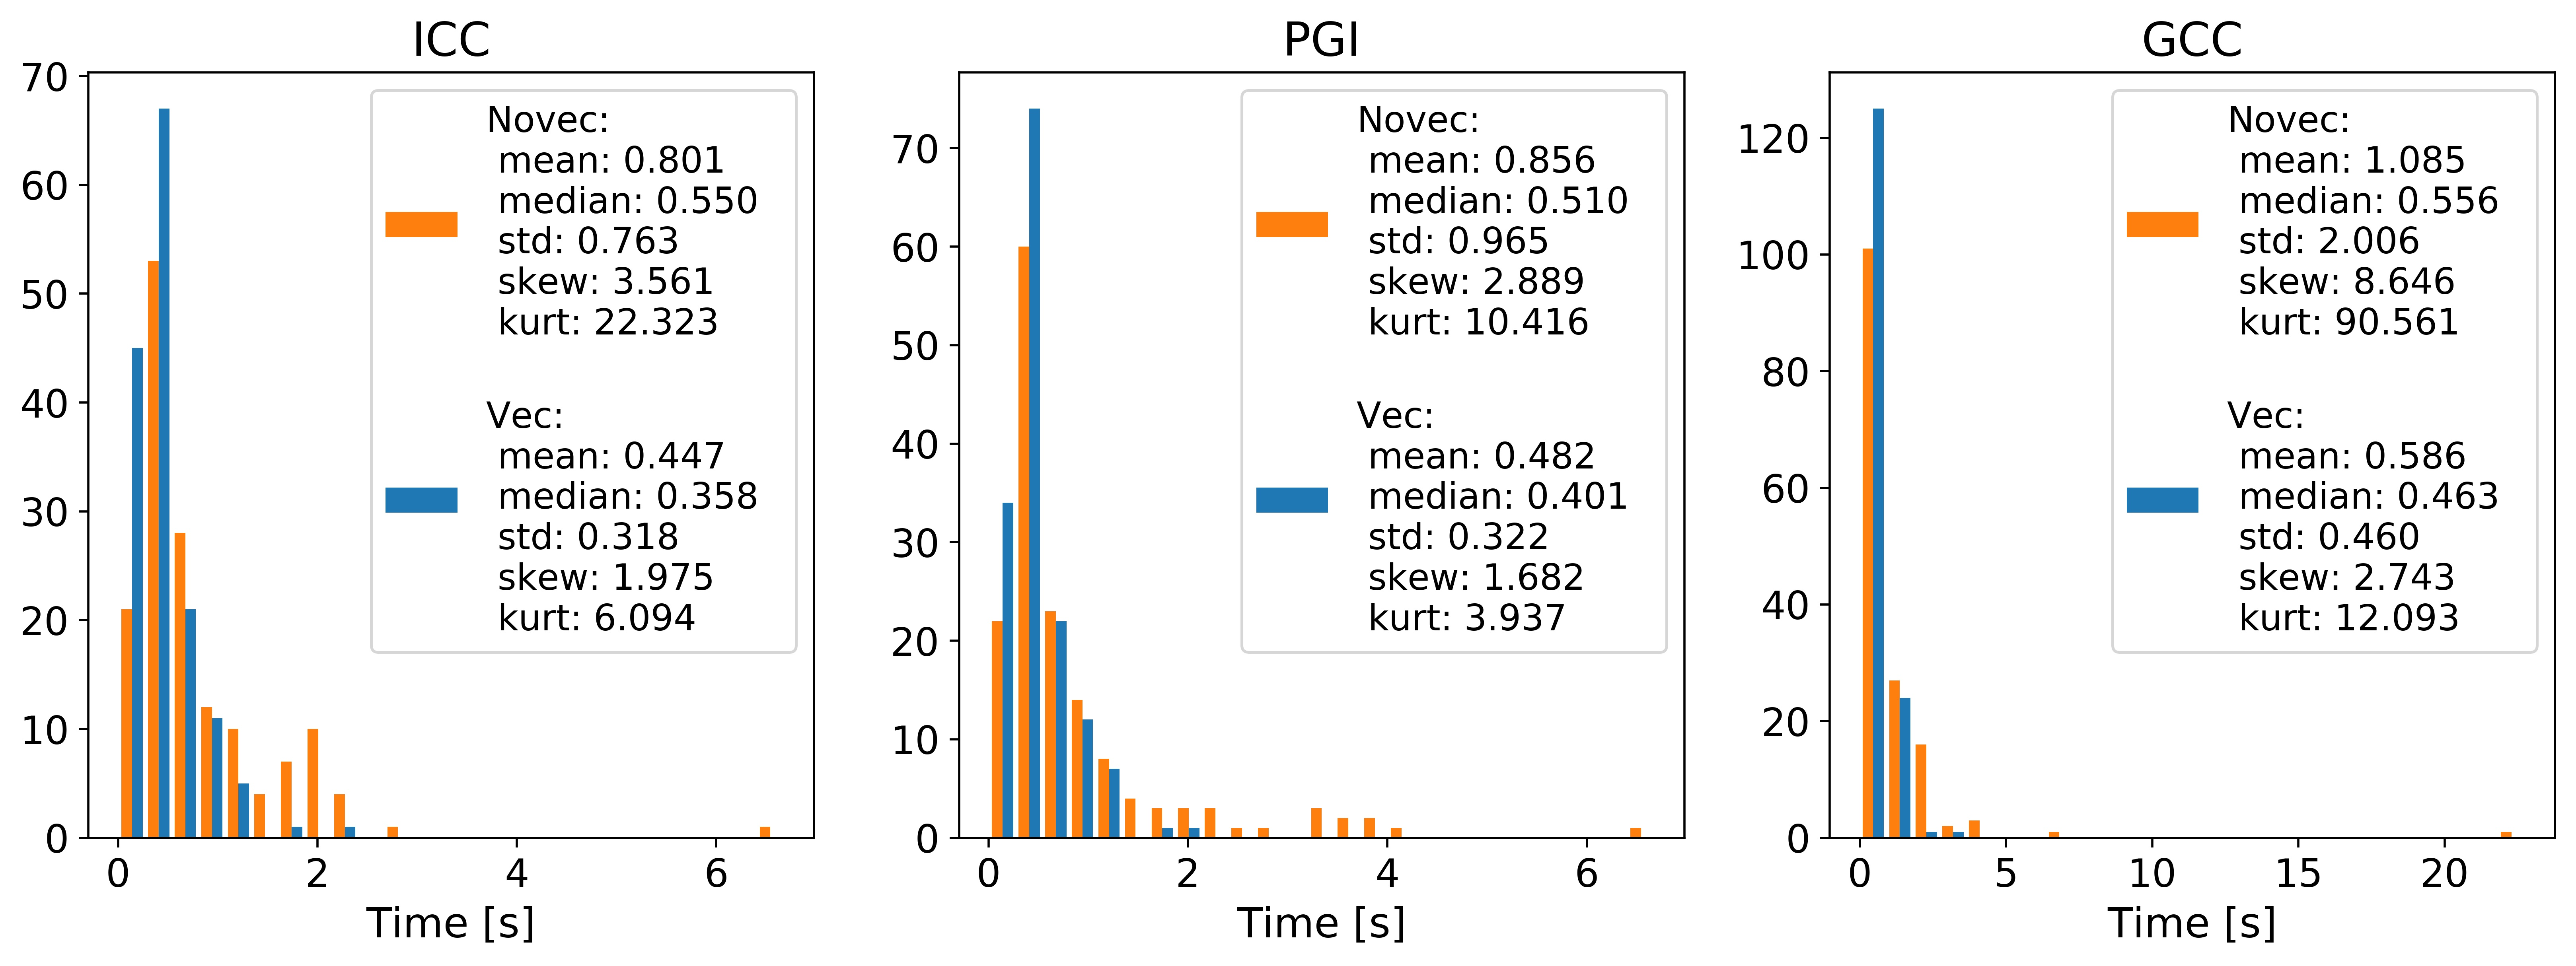
\includegraphics{Figuras/stats2.jpg}}		
	\end{center}
	\vspace{2mm}	% acrescentar o espaçamento vertical apropriado entre a borda inferior da figura e a legenda ou a fonte quando não há legenda (o valor pode ser negativo para subir)
	\caption{Histogramas e estatísticas dos resultados obtidos com as novas flags de compilação. O número de bins é igual a 25.}
	\legenda{}	% legenda - para deixar sem legenda usar comando \legenda{} (nunca deve-se comentar o comando \legenda)
	\label{fig:2_hist}
%	\FONTE{FOnte da imagem (se necessário).}	% fonte consultada (elemento obrigatório, mesmo que seja produção do próprio autor)
\vspace{-8mm}
\end{figure}


\begin{table}[H]
\center
\caption{\textit{Speedups} médios após as novas flags de compilação e seus  $\delta$'s.} 
\begin{tabular}{@{}l l l l@{}}
\toprule
& \texttt{ICC} & \texttt{PGI} &  \texttt{GCC} \\
\midrule
\textit{Speedup} médio & 1.83 & 2.00 & 1.971 \\ 
Alteração relativa ($\delta$) & $+1.1\%$ & $+2.1\%$ & $+39.7\%$ \\ 
\bottomrule
\end{tabular}
\label{tab:2_spedups}
\vspace{-10mm}
\end{table}


\begin{table}[H]
\center
\caption{Tempos totais com as novas flags de compilação seus $\delta$'s.} 
\vspace{-4mm}
\begin{tabular}{@{}l l l l l l l l l@{}}
\toprule
& \multicolumn{2}{@{}c@{}}{\texttt{ICC}} & & \multicolumn{2}{@{}c@{}}{\texttt{PGI}} & &  \multicolumn{2}{@{}c@{}}{\texttt{GCC}} \\
\cmidrule{2-3} \cmidrule{5-6} \cmidrule{8-9}
& Não-vet. & Vet.  & &  Não-vet. & Vet.  & &  Não-vet. & Vet. \\
\midrule
Tempo total [s] & 120.891 &  67.476 & & 129.241 &  72.834 & &  163.855  &  88.499  \\
Alteração relativa ($\delta$) & $0\%$ &  $-0.6\%$ & & $+1\%$ &  $-1.2\%$ & &  $-1.9\%$ & $-34.7\%$ \\
\bottomrule
\end{tabular}
\label{tab:2_tempos}
\vspace{-10mm}
\end{table}


\begin{table}[H]
\center
\caption{Número de loops vetorizados e não-vetorizados (diferença com relação ao resultado anterior entre parênteses).}
\begin{tabular}{@{}l l l l l l l l@{}}
\toprule
\multicolumn{2}{@{}c@{}}{\texttt{ICC}} & & \multicolumn{2}{@{}c@{}}{\texttt{PGI}} & &  \multicolumn{2}{@{}c@{}}{\texttt{GCC}} \\
\cmidrule{1-2} \cmidrule{4-5} \cmidrule{7-8}
Não-vet. & Vet.  & &  Não-vet. & Vet.  & &  Não-vet. & Vet. \\
\midrule
53    &    98 (+4)   &&     99     &    52  (+2)   &&     92   & 59 (+16) \\
\bottomrule
\end{tabular}
\label{tab:2_nloops}
\end{table}
%\begin{figure}[ht!]
%	\caption{Caption: figure example.}
%	\vspace{0mm}	% acrescentar o espaçamento vertical apropriado entre o título e a borda superior da figura
%	\begin{center}
%		\resizebox{13cm}{!}{\includegraphics{Figuras/jpg_omni2_daily_wSxReptBqw.jpg}}		
%	\end{center}
%	\vspace{-2mm}	% acrescentar o espaçamento vertical apropriado entre a borda inferior da figura e a legenda ou a fonte quando não há legenda (o valor pode ser negativo para subir)
%	\legenda{Legend.}	% legenda - para deixar sem legenda usar comando \legenda{} (nunca deve-se comentar o comando \legenda)
%	\label{figfiltrotS0681200}
%	\FONTE{FOnte da imagem (se necessário).}	% fonte consultada (elemento obrigatório, mesmo que seja produção do próprio autor)
%\end{figure}



\newpage
%%%%%%%%%%%%%%%%%%%%%%%%%%%%%%%%%%%%%%%%%%%%%%%%%%%%%%%%%%%%%%%%%%%%%%%%%%%%%%%

\chapter{CONCLUSÕES}
\label{chp:3}

\vspace{4mm}
\textbf{Conclusões da Seção I}\vspace{6mm}\\
A partir dos resultados apresentados na Seção \ref{chp:1}, conclui-se sobre a performance individual dos compiladores:
\begin{itemize}
\item Os tempos médios (Figura \ref{fig:a}) e totais (Tabela \ref{tab:d}) das versões vetorizada e não-vetorizada foram menores para o compilador \texttt{ICC}. Apesar dessa performance superior no geral, ele obteve um \textit{Speedup} médio intermediário (Tabela \ref{tab:c}); este foi o compilador que vetorizou o maior número de loops (Tabela \ref{tab:e}).
%
\item O \textit{Speedup} médio do compilador \texttt{PGI} foi o maior dentre os compiladores testados; enquanto seus tempos totais se aproximam dos valores do compilador \texttt{ICC} (Tabela \ref{tab:d}), seu número de loops vetorizados e não-vetorizados é comparável ao do \texttt{GCC} (Tabela \ref{tab:e}).
%
\item Conforme indicado pela alta assimetria e curtose dos tempos obtidos com o \texttt{GCC}, a performance geral deste compilador foi penalizada pela presença de um loop que durou acima de 20 segundos (Figura \ref{fig:a}, plot da direita); este foi o compilador com menor \textit{Speedup} médio e piores tempos totais.
\end{itemize}

Sobre a capacidade de vetorização dos três compiladores, o diagrama de Venn da Figura \ref{fig:f} revela que:
\begin{itemize}
\item \texttt{ICC} foi o compilador que exclusivamente vetorizou o maior número de loops: 27 ($17.9\%$ do total), contra 4 ($2.6\%$ do total) tanto do \texttt{PGI} quanto do \texttt{GCC}.
\item Somente 10 loops foram vetorizados por todos os compiladores, ou seja, $6.6\%$ dos 151 loops de teste;
\item 45 loops não foram vetorizados por nenhum compilador, representando $29.8\%$ dos loops de teste.
\end{itemize}

\textbf{Conclusões da Seção II}\vspace{6mm}\\
Com relação aos resutados obtidos na Seção \ref{chp:2}, destaca-se:
\begin{itemize}
\item \texttt{ICC} teve somente sua flag de vetorização alterada; \texttt{PGI} teve tanto sua flag de otimização base quanto a de vetorização alteradas; \texttt{GCC} teve somente sua flag de otimização base alterada (ver Tabela \ref{tab:2_flags}).
%
\item Todos os compiladores aumentaram seus \textit{Speedups} médios; dito isto, \texttt{GCC} foi o compilador que apresentou a maior alteração nos resultados; de fato, seu \textit{Speedup} médio superou o do \texttt{ICC} (Tabela \ref{tab:2_spedups}) e seu número de loops vetorizados superou o do \texttt{PGI} (Tabela \ref{tab:2_nloops}).
%
\item A nova flag de otimização base utilizada para o compilador \texttt{GCC} melhorou a performance da versão não-vetorizada (redução de $1.9\%$ do tempo total), enquanto ofereceu um ganho ainda maior para a versão vetorizada (redução de $34.7\%$ do tempo total), conforme mostra a Tabela \ref{tab:2_tempos}; a Figura \ref{fig:2_hist}, plot da direita, indica que a assimetria e a curtose diminuíram significativamente com a eliminação da amostra com mais de 20 segundos na versão vetorizada.
%
\item \texttt{PGI} foi o compilador que obteve o menor número de novos loops vetorizados: +2, contra +4 do \texttt{ICC} e +16 do \texttt{GCC} (Tabela \ref{tab:2_nloops}).
%
\item Mesmo o \texttt{ICC} apresentando a melhora menos significativa de \textit{Speedup} médio, obtendo $+1.1\%$ contra $+2.1\%$ do \texttt{PGI} e $+39.7\%$ do \texttt{GCC} (Tabela \ref{tab:2_spedups}), ele permaneceu como o compilador com menores tempos tanto na versão vetorizada quanto na versão não-vetorizada (Figura \ref{fig:2_hist} e Tabela \ref{tab:2_tempos}). 
%
\item O número de loops vetorizados por todos os compiladores subiu de 10 para 24, que representa $15.8\%$ do total. 
%
\item O número de loops não vetorizados por nenhum compilador caiu de 45 para 40, representando agora $26.8\%$ do total. A interseção destes dois conjuntos é igual a 39, ou seja, os compiladores não foram capazes de vetorizar 39 loops em nenhum dos casos.
\end{itemize}
%\begin{figure}[ht!]
%	\caption{Caption: figure example.}
%	\vspace{0mm}	% acrescentar o espaçamento vertical apropriado entre o título e a borda superior da figura
%	\begin{center}
%		\resizebox{13cm}{!}{\includegraphics{Figuras/jpg_omni2_daily_wSxReptBqw.jpg}}		
%	\end{center}
%	\vspace{-2mm}	% acrescentar o espaçamento vertical apropriado entre a borda inferior da figura e a legenda ou a fonte quando não há legenda (o valor pode ser negativo para subir)
%	\legenda{Legend.}	% legenda - para deixar sem legenda usar comando \legenda{} (nunca deve-se comentar o comando \legenda)
%	\label{figfiltrotS0681200}
%	\FONTE{FOnte da imagem (se necessário).}	% fonte consultada (elemento obrigatório, mesmo que seja produção do próprio autor)
%\end{figure}





%\include{./docs/conclusion}


%% insira quantos capítulos desejar com o seguinte comando:
%\include{_pasta_do_arquivo_/_meu_arquivo_} %%sem a extensão
%% note que deverá haver um arquivo _meu_arquivo_.tex (com extensão) no diretório _pasta_do_arquivo_

%\include{./docs/conclusao}

%% Bibliografia %% não alterar %% obrigatório %testebib
\bibliography{./bib/referencia} %% aponte para seu arquivo de bibliografia no formato bibtex (p.ex: referencia.bib)


%\include{./docs/glossario} %% insira os termos do glossário no arquivo glossario.tex %% opcional

%\inicioApendice %% opcional, comente esta linha e a seguintes se não houver apendice(s)
%\include{./docs/apendice1} %% insira apendices tal qual capítulos acima


%\inicioAnexo
%\include{./docs/anexo}
%\include{./docs/anexo1}
%\include{./docs/anexo2}

%\inicioIndice
%\include{./docs/contracapa}
\end{document}